\section{Background And Motivation}
\label{bkg_motivation}

\subsection{Background}
\label{bkg}



\subsection{Personalized Features \textit{\textbf{\large}}}
\label{feature}
In this paper, we consider five kinds of contextual information as follows:




\begin{itemize}
    \item \textbf{$L$:} 

    \item \textbf{$D, H$:} 

    \item \textbf{$Wf$:} 

    \item \textbf{$B, C$:} 

    \item \textbf{$LP$:} 
\end{itemize}


 Table~\ref{tbl: acronym} summarizes the features considered. What's more, the table also give the description of acronyms to be used in the following passage.


\subsection{Traditional Bayesian Algorithm \textit{\textbf{\large}}}
\label{traditional_algorithm}
 The traditional Bayesian algorithm is shown in Equation~\ref{eq: prediction}, we calculate each App's prediction score given the context by multiplying the CPDs(the conditional probability distribution) of the App and each context. Then the top scored Apps are the final predictions. The CPD $P(A | C)$ denote that the probablity of launching an App under the condition of the last used App. The meaning of the other three CPDs is similar.


\begin{table}[t]
\setlength{\tabcolsep}{1.2em}
\scriptsize
  \centering
  \caption{Notation used in this paper.}
  %\begin{tabular}{|p{3cm}<\centering||p{1.2cm}<\centering|p{2cm}<\centering|p{2cm}<\centering|p{2cm}<\centering|}
  \begin{tabular}{c|c}
     \hline
     Symbol & Description \\
     \hline
     \hline
     $L$ & the location  \\
     $D$ & day of week  \\
     $H$ & hour of day  \\
     $Wf$ & the rate level of wifi  \\
     $B$ & the battery level  \\
     $C$ & a flag whether the battery is being charged  \\
     $LP$ & the latest used App  \\
     $A$ & the App   \\
     $CPD$ & the conditional probability distribution  \\
     \hline
   \end{tabular}
 \label{tbl: acronym}
 \vspace{-0.1in}
\end{table}


\begin{equation}
\footnotesize
\label{eq: prediction}
    Socre(A) = P(A | C) \times P(A|D,H,L) \times P(A|W) \times P(A|U)
\end{equation}


 It is intuitive that we should consider as many records (i.e., training data) as possible in order to achieve high prediction accuracy. Because the penalty for using small training sets is over fitting: while in-sample performance may be excellent, The previous work on App prediction has tended to make use of a lot of training samples. However, we need to take the specific area of application into account. Using machine learning algorithm to predict next App that smartphone user will be used, we have to consider that user behavior patterns can have a change gradually. Thus, using long-term training sets can reduce prediction accuracy instead.


\begin{figure}[t]
    \centering
    \begin{tabular}[t]{c}
        \subfloat[]{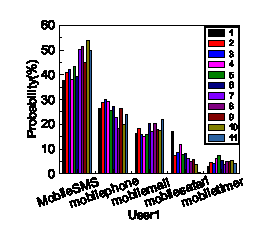
\includegraphics[width=0.55\columnwidth]{fig/U1_5_5_frequency.eps}}
        \subfloat[]{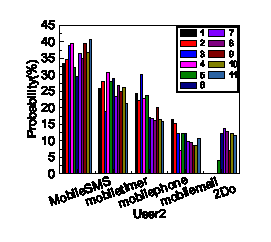
\includegraphics[width=0.55\columnwidth]{fig/U2_5_5_frequency.eps}}
    \end{tabular}
    \centering
    \begin{tabular}[t]{c}
        \subfloat[]{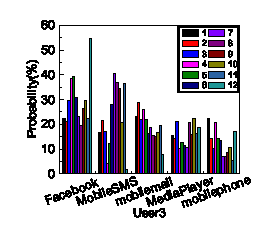
\includegraphics[width=0.55\columnwidth]{fig/U3_5_5_frequency.eps}}
        \subfloat[]{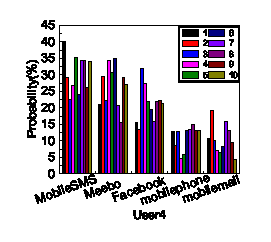
\includegraphics[width=0.55\columnwidth]{fig/U4_5_5_frequency.eps}}
    \end{tabular}
    \caption{(a)(b)(c)(d)indicate that the used ratio of most frequently used 8 Apps on four different smartphone users.}
    \label{fig: motivation}
    \vspace{-0.1in}
\end{figure}


To demonstrate our inference, we have an analysis of most frequently used Apps. As shown in Figure~\ref{fig: motivation}, we count the used ratio of 8 Apps every 5 weeks. The number of tag such as 2 indicates the second five- weeks in the upper right corner. The 8 Apps are the most frequently used Apps for the user. The used ratio of every App varies with time. Thus, in term of the used frequency of Apps, we conclude the conclusion that user behavior pattern of using Apps varies with time.

\begin{figure}[t]
    \centering
    \begin{tabular}[t]{c}
        \subfloat[]{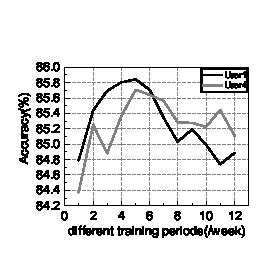
\includegraphics[width=0.55\columnwidth]{fig/U1_U4.eps}}
        \subfloat[]{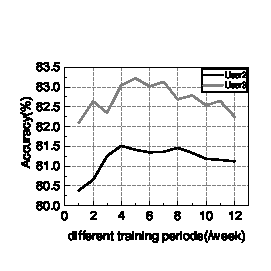
\includegraphics[width=0.55\columnwidth]{fig/U2_U3.eps}}
    \end{tabular}
    \caption{(a)(b)indicate that the changing trend of prediction accuracy along with increasement of the size of training sets.}
    \label{fig: 2_week_test_accuracy}
    \vspace{-0.1in}
\end{figure}



Also, we demonstrate the inference from the view of the prediction accuracy. We explore the impact of the amount of training data ranged from one week to twelve weeks on the prediction accuracy. There are two schemes to get prediction accuracy from data set. The two schemes are shown in Figure ~\ref{fig: train_test_flow}. In Scheme 1, training periods and test periods alternately present and they have no overlap on the time dimension. From Figure ~\ref{fig: train_test_flow}(b), we can find that there exists overlapping parts on the time dimension in Scheme 2. And in Scheme 2, there is no time interval in two adjacent test periods. In both two schemes, after the $i_{th}$ training period, we get prediction accuracy from the corresponding $i_{th}$ test period based on the model trained in the $i_{th}$ training period. In the Equation~\ref{eq: user_acc}, $ave_acc_user$(the average value of all the average accuracy in every test period) represent the prediction accuracy on a user and $acc\_each$ is the prediction accuracy each test. $n_{1}$ is the number of test periods in dataset and $n_{2}$ is the times of test in each test period.


\begin{equation}
\footnotesize
\label{eq: user_acc}
ave\_acc\_user=\sum_{i=1}^{n_{1}} \sum_{j=1}^{n_{2}} acc\_each
\end{equation}


In this paper, we adopt


\begin{figure}[t]
    \centering
    \begin{tabular}[t]{c}
        \subfloat[]{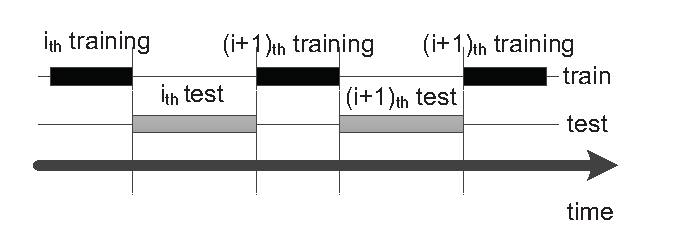
\includegraphics[width=0.95\columnwidth]{fig/train_test_flow_scheme1.eps}}
    \end{tabular}
    \centering
    \begin{tabular}[t]{c}
        \subfloat[]{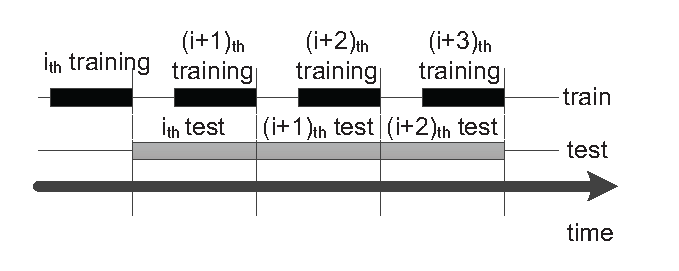
\includegraphics[width=0.95\columnwidth]{fig/train_test_flow_scheme2.eps}}
    \end{tabular}
        \caption{(a) (b) represents two different schemes to get prediction accuracy from data set. (a) describes Scheme 1 and (b) describe Scheme 2.}
    \label{fig: train_test_flow}
\end{figure}


As shown in Figure~\ref{fig: 2_week_test_accuracy}, the experimental results are based real traces collected from the 9 participants. And the k is set at 5. From the Figure~\ref{fig: 2_week_test_accuracy}, we can see that the prediction accuracy will rise at the beginning, but it will drop then. Namely, the accuracy is saturated at certain point from one week to twelve week. Therefore, the long-term training data does not necessarily achieve higher accuracy. Heuristically, it is because mobile users may install new Apps and have changed their behavior patterns(e.g. preferences) slightly. On the other hand, more records(i.e., training data) more time required to make prediction.


We also conclude from Figure~\ref{fig: 2_week_test_accuracy} that the positions the saturation points varies greatly on different mobile users. So it is necessary to have s adaptive scheme to adjust the amount of training data. However, it is difficult to select the optimal amount of training data directly. The work flow of App prediction is training-prediction-retraining-reprediction. We fixed the amount of training data and adjust the time span of the period of prediction instead. Because the precision accuracy is easily obtained in the period of prediction. We can adjust the time span based on the prediction accuracy.


From Figure~\ref{fig: motivation,fig: 2_week_test_accuracy}, we get two observations that provide useful insights into the design of our algorithm.


\textbf{Observation 1:}User behavior pattern of using Apps varies with time. And the recent used Apps are more useful to predict the next used Apps.


\textbf{Observation 2:}For different smartphone users, the optimal amounts of training data id different. Therefore, we propose an adaptive algorithm to solve the problem.

%Instead, select an approximate time span of p


%On the one hand, more records(e.g. train

%Different size of training sets are chosento measure the influence of the size of training sets on prediction accuracy. We do our experiments on nine smartphone users. According to the time span of training sets, the training sets is classified into twelve categories. The time span of twelve categories is from one week to twelve week. The experimental results are shown in the Figure~\ref{fig: 2_week_test_accuracy}.

%we first count the 8 Apps of most frequently used Apps from the whole datasets from different users. Then, the used ratio


%In addition, predicting mobile application usage with contextual information has been studied for a long time. Ke Huang et al~\cite{PredictByContextInfo} study bayes based method and linear model to conduct prediction. And ~\cite{PredictTLB} proposes a prediction-guided multi-grain TLB design that uses a superpage prediction mechanism to avoid multiple lookups in the common case.

%As a result, processes are terminated directly if there is no enough memory space, which may degrade user satisfaction.


\subsection{Adjusting the time span of the prediction period adaptively \textit{\textbf{\large}}}
\label{measure_study}
%\subsection{Launching Apps with Swapping: \textit{\textbf{\large Not}} Just Read I/O!}
%\label{measure_study}
From the above, choosing an approximate amount of training data can not only improve the prediction accuracy but also reduce the time required to train the prediction model. Because the prediction accuracy can be obtained in the period of prediction, we choose an a dynamic time span of prediction period instead of a dynamic amount of training data. We thus propose a strategies based on the minimization of the prediction error. It can be considered as \emph{early stopping}.


\emph{Early stopping}: In machine learning, early stopping is a form of regularization used to avoid over-fitting when training a learner with an iterative method, such as gradient descent. Such methods update the learner so as to make it better fit the training data with each iteration. Early stopping rules provide guidance as to how many iterations can be run before the learner begins to over-fit.


We have used the strategy of \emph{early stopping} to achieve the adaptive time span of prediction periods. The detailed description is as follows. After training with a fixed amount of training data, the achieved model by training is used to predict the Apps that will be used next. At this time, an approximate time span of prediction periods need to be considered. Too long time span of prediction periods can make the prediction accuracy decreased. But too short time span of prediction periods can increase the training costs(i.e., more training times are needed). In our strategy of \emph{early stopping}, we first need to selected an initial time interval(e.g., two weeks). In the strategy, the shortest time span of prediction period is one week(i.e., the first week in the two weeks). The rest of the prediction time can be dynamically adjusted. Except from the first week, the average precision accuracy(acc\_day) of the whole prediction period need to be calculated with every passing day. At the same time, the average prediction accuracy(acc\_week) of the whole prediction period also need to be calculated with every passing week. But considering to improve the final prediction accuracy, the maximal acc\_week(max\_acc\_week) is chosen as a baseline.


Intuitively, the acc\_week is more stable than the acc\_day, and the it is more representative than the acc\_day. Thus, with every passing day, we calculate acc\_day, max\_acc\_week and compare acc\_day and max\_acc\_week. Provided the ratio of acc\_day and acc\_week is less than the threshold that we set, we have a time penalty for time span of prediction period(i.e., reducing the time span of prediction period). In the beginning, we have selected an initial time interval of two week. Excluding the first week, the second week is chosen as a baseline. When the prediction accuracy is too low, the time span of prediction period can be reduced on the basis of the baseline.


\begin{algorithm}[!t]
\SetKwInOut{Input}{Input}\SetKwInOut{Output}{Output}
\footnotesize
 \Input{$L$: an empty list;
        $TS$: a fixed time span;
        $Thres1$: a number between 0 and 1;
        $Thres2$: a number between 0 and 1;}
 \Output{$ave\_acc_{total}$: the average prediction accuracy in the whole prediction period;}
 \medskip
 $n\_predict$ $\leftarrow$ 0\;
 $sum\_accuracy$ $\leftarrow$ 0\;
  \For{each $TS$ in the firstweek of the prediction period}{
    Predict next used Apps and get the prediction accuracy $P$\;
    $n\_predict$ $\leftarrow$ $n\_predict$+1\;
    $sum\_accuracy$ $\leftarrow$ $sum\_accuracy$+$P$\;
    \If{$Sum$ is an integer multiple of one day}{
        Add the tuple ($n\_predict$,$sum\_precision$) into list $L$\;
        $n\_predict$ $\leftarrow$ 0\;
        $sum\_accuracy$ $\leftarrow$ 0\;
    }
  }
  $RS$: the rest of prediction period;
  $RS$ $\leftarrow$ the time of one week;
  $n\_predict$ $\leftarrow$ 0\;
  $sum\_accuracy$ $\leftarrow$ 0\;
  $flag$: a flag on whether to increase the time of prediction period\;
  $flag$ $\leftarrow$ \emph{True}
  \While{$flag$}{
      \For{each $TS$ in $RS$}{
        Predict next used Apps and get the prediction accuracy $P$\;
        $n\_predict$ $\leftarrow$ $n\_predict$+1\;
        $sum\_accuracy$ $\leftarrow$ $sum\_accuracy$+$P$\;
        \If{$Sum$ is an integer multiple of one day}{
            Add the tuple ($n\_predict$,$sum\_precision$) into list $L$\;
            $n\_predict$ $\leftarrow$ 0\;
            $sum\_accuracy$ $\leftarrow$ 0\;
            Calculate average accuracy $ave_acc$ according to $L$\;
            Get the maximal accuracy $max_acc$ in the first one,two,... of prediction period
            \If{$ave\_acc$ < $max_acc$ $\times$ $Thres1$}{
                Have a penalty for $ave\_acc$(lowering the value)\;
            }
        }
      }
      Calculate average accuracy $ave_acc$ according to $L$\;
      Get the maximal accuracy $max_acc$ in the first one,two of prediction period\;
      \If{$ave\_acc$ > $max\_acc$ $\times$ $Thres2$}{
        Have an award for $RS$ (add the value)\;
      }
      $flag$ $\leftarrow$ \emph{False}\;
  }
  Calculate $ave\_acc_{total}$ according to $L$\;
  \Return $ave\_acc_{total}$;
  \caption{\textsc{Early Stopping Algorithm}}
 \label{alg: early stopping}
 \vspace{-0.2in}
\end{algorithm}


In the Algorithm\ref{alg: early stopping}, the penalty function \emph{penal\_func} is the key. We have tried to use different formula. After a lot of experiments, we choose Formula\ref{eq: penalty_function} as our final penalty function. In Formula\ref{eq: penalty_function}, $threshold$ is a number between 0 and 1 and $a$ is a parameter. Heuristically, the rate of growth of the logarithmic function value is more and more gentle, which will effectively avoid certain accidental factors to reduce the time interval between two adjacent training.

\begin{equation}
\footnotesize
\label{eq: ratio_function}
ratio=\frac{\sum_{i=1}^n each\_acc}{n \times max\_ave\_acc}
\end{equation}


\begin{equation}
\footnotesize
\label{eq: penalty_function}
    penalty=1+\frac{log(threshold)-log(ratio)}{log(a)}
\end{equation}


\begin{figure}[t]
    \centering
    \begin{tabular}[t]{c}
        \subfloat[]{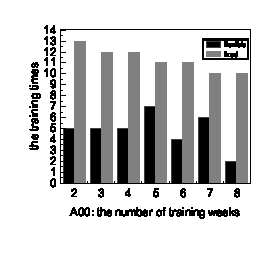
\includegraphics[width=0.55\columnwidth]{fig/A00_trainingtimes.eps}}
    \end{tabular}
    \caption{(a)(b)indicate that the changing trend of prediction accuracy along with increasement of the size of training sets.}
    \label{fig: training_times}
    \vspace{-0.1in}
\end{figure}


As shown in Figure\ref{fig: training_times}, our adaptive method nearly reduce half of the training times with flexible prediction period than using fixed prediction period(two weeks). In addition, in terms of the accuracy, the adaptive method nearly obtains the same prediction accuracy and even has an improvement for some users. The accuracy result of comparison is listed in Table \ref{tbl: adaptive_accuracy}.



\begin{table}[t]
\setlength{\tabcolsep}{.3em}
\scriptsize
  \centering
  \caption{the result of accuracy comparison between our adaptive method and adopting fixing prediction period method.}
  %\begin{tabular}{|p{3cm}<\centering||p{1.2cm}<\centering|p{2cm}<\centering|p{2cm}<\centering|p{2cm}<\centering|}
  \begin{tabular}{|c|c|c|c|c|c|c|c|c|c|}
     \hline
      \multirow{2}{*}{User} & \multirow{2}{*}{Strategy} & \multicolumn{7}{c|}{training weeks(/week)} & \multirow{2}{*}{avg} \\
      \cline{3-9}
      & & \tabincell{c}{2} & \tabincell{c}{3} & \tabincell{c}{4} & \tabincell{c}{5} & \tabincell{c}{6} & \tabincell{c}{7} & \tabincell{c}{8} & {}\\
      \hline
      \hline
      \multirow{2}{*}{A00} & \tabincell{c}{flexible(\%)} & \tabincell{c}{84.86} & \tabincell{c}{84.30} & \tabincell{c}{84.57} & \tabincell{c}{84.77} & \tabincell{c}{84.57} & \tabincell{c}{84.77} & \tabincell{c}{84.03} & \tabincell{c}{84.55}\\
      \cline{2-10}
      & \tabincell{c}{fixed(\%)} & \tabincell{c}{83.89} & \tabincell{c}{84.48} & \tabincell{c}{83.78} & \tabincell{c}{84.25} & \tabincell{c}{84.21} & \tabincell{c}{84.04} & \tabincell{c}{84.11} & \tabincell{c}{84.11}\\
      \hline
      \multirow{2}{*}{A03} & \tabincell{c}{flexible(\%)} & \tabincell{c}{89.58} & \tabincell{c}{89.51} & \tabincell{c}{89.58} & \tabincell{c}{89.53} & \tabincell{c}{89.51} & \tabincell{c}{89.54} & \tabincell{c}{89.64} & \tabincell{c}{89.55}\\
      \cline{2-10}
      & \tabincell{c}{fixed(\%)} & \tabincell{c}{89.51} & \tabincell{c}{89.22} & \tabincell{c}{89.07} & \tabincell{c}{89.38} & \tabincell{c}{89.53} & \tabincell{c}{89.59} & \tabincell{c}{89.64} & \tabincell{c}{89.42}\\
      \hline
   \end{tabular}
 \label{tbl: adaptive_accuracy}
 \vspace{-0.1in}
\end{table}

%In Figure~\ref{fig: sys_arch}, \emph{watcher} monitors memory capacity variation, and performs early page swap to reduce the swapping probability during application launch procedure. The candidate pages to be swapped out are indicated by launching \emph{predictor} in Figure~\ref{fig: sys_arch}. \emph{Predictor} performs application prediction based on a user's behavior and context feature, such as time, location, the usage of the mobile device and so on. In addition, if low memory condition occurs again during user's interaction with the mobile device, \emph{watcher} would send commands to LMK unit in kernel space to kill processes based on their priority and the prediction result of \emph{predictor}.

%Our work distinguishes from most of the previous work in two aspects: 1) the optimization is based on the original architecture, which make it practical, 2) design and evaluate our system from user's perspective. Furthermore, different from previous work, our work predicts the most rarely used application list to be swapped out to adjust the amount of free memory ahead-of-time. Thus, the prediction accuracy is high enough (more than 90\%) to conduct process swapping.
